\documentclass[fleqn,10pt]{wlscirep}
% wlscirep.cls available from Overleaf: search "Scientific Reports" template

% ─── PACKAGES ───────────────────────────────────────────────────
\usepackage[utf8]{inputenc}
\usepackage[T1]{fontenc}
\usepackage{subcaption}
\usepackage{caption}
\usepackage{float}
\usepackage{placeins}
\usepackage{booktabs}
\usepackage{siunitx}
\usepackage{amsmath}
\usepackage{graphicx}
\usepackage{microtype}
\usepackage{tikz}
\usetikzlibrary{arrows.meta,positioning}

% ─── SUPPLEMENTARY FIGURE COUNTER ───────────────────────────────
\makeatletter
\@ifundefined{c@suppfigure}{\newcounter{suppfigure}}{}
\makeatother
\renewcommand{\thesuppfigure}{S\arabic{suppfigure}}

% ─── HYPERREF ───────────────────────────────────────────────────
\usepackage{hyperref}
\hypersetup{
    colorlinks=true,
    linkcolor=blue,
    citecolor=blue,
    urlcolor=blue
}

% ─── TITLE & AUTHORS ────────────────────────────────────────────
\title{Topical dental anesthesia induces transient masseter EMG amplitude gain
       without altering masticatory rhythm: a within-subject secondary analysis}

\author[1,2,*]{Sebastian Espinoza}
\author[3,4]{Daniel Moraga-Espinoza}
\author[4]{Luis Morreal-Ortega}
\author[1,5]{Wael El-Deredy}

\affil[1]{Brain Dynamics Lab, Interdisciplinary Center of Biomedical and Engineering
          Research for Health, Universidad de Valpara\'{i}so, Chile.}
\affil[2]{Dentistry School, Universidad de Valpara\'{i}so, Chile.}
\affil[3]{Chemistry and Pharmacy School, College of Pharmacy, Universidad de
          Valpara\'{i}so, Chile.}
\affil[4]{Center for Research, Development and Innovation of Bioactive Products
          (CInBIO), Universidad de Valpara\'{i}so, Chile.}
\affil[5]{School of Biomedical Engineering, Universidad de Valpara\'{i}so, Chile.}
\affil[*]{sebastian.espinoza@uv.cl}

\keywords{Mastication; electromyography; topical anesthesia; sensorimotor
          compensation; central pattern generator; oral somatosensory feedback;
          masseter}

\begin{abstract}
Masticatory motor output depends on continuous periodontal and mucosal
somatosensory feedback mediated by trigeminal afference.
Whether the motor system compensates for transient reduction of this feedback
has not been rigorously characterised.
We present a secondary electromyographic (EMG) analysis of a within-subject
crossover dataset ($N$\,=\,34) in which unilateral topical lidocaine (10\%) or
matched placebo spray was applied before four 60-second chewing bouts occurring
at approximately 3, 7.5, 12, and 17~min post-application.
Masseter activity was recorded bipolarly at 1024~Hz, filtered 20--450~Hz with
Zapline-plus line-noise suppression, and analysed bout-by-bout using paired
Wilcoxon tests with Benjamini--Hochberg correction and repeated-measures ANOVA.
Session-averaged comparisons across all four bouts showed no significant
differences for any metric (equivalence confirmed by two one-sided tests at
$d$\,=\,0.5).
Resolving by bout revealed a time-dependent effect: at bout~1
($\approx$3~min post-application, maximal anesthesia), median cycle amplitude
was greater under anesthesia ($d_z$\,=\,0.695, $p$\,=\,0.0003,
Benjamini--Hochberg FDR-corrected $p$\,=\,0.0035), alongside increases in
RMS amplitude, total power, and spectral power in 20--150~Hz bands
(all FDR-corrected $p$\,<\,0.03) and greater inter-cycle regularity
(CV of inter-peak interval $d_z$\,=\,$-$0.434, FDR $p$\,=\,0.042).
These effects decayed monotonically across bouts~2--4 (trend $p$\,=\,0.0002),
consistent with topical lidocaine washout.
Critically, median frequency, chewing rate, and duty cycle showed no change at
any bout (non-significant at all time points; two one-sided test equivalent).
Cycle-locked time-frequency analysis identified a broadband cluster
($\approx$30--300~Hz) of greater EMG power under anesthesia at bout~1
(cluster permutation $p$\,=\,0.035 directional; two-tailed $p$\,=\,0.051),
absent at bout~4.
These results indicate that transient oral somatosensory deprivation elicits
sensorimotor gain compensation in the masseter -- greater amplitude and
regularity without timing change -- consistent with a hierarchical model in
which the brainstem central pattern generator maintains rhythm while peripheral
feedback modulates efferent gain.
This preserved rhythmic output provides a post-hoc manipulation check for the
parent study and a mechanistic account of why the cognitive and cortical effects
of chewing are unaffected by dental anesthesia.
\end{abstract}

% ─── BILINGUAL ABSTRACT (Spanish — for departmental records; not for SR submission) ───
%
% \begin{abstract}[Resumen]
% La actividad motora masticatoria depende de la retroalimentación somatosensorial
% periodontal y mucosa mediada por la vía trigeminal. No se ha caracterizado
% rigurosamente si el sistema motor compensa la reducción transitoria de esta
% retroalimentación. Presentamos un análisis electromiográfico secundario de un
% conjunto de datos cruzados intrasujeto ($N$\,=\,34) en el que se aplicó
% lidocaína tópica unilateral (10\%) o spray placebo equivalente antes de cuatro
% series de masticación de 60~s a $\approx$3, 7,5, 12 y 17~min post-aplicación.
% El análisis muestra que la amplitud del ciclo masticatorio fue mayor bajo
% anestesia en la primera serie ($d_z$\,=\,0{,}695, $p_{\text{FDR}}$\,=\,0{,}0035),
% sin cambios en frecuencia, tasa o ciclo de trabajo, con decaimiento consistente
% con el lavado farmacológico de la lidocaína. Estos resultados indican que la
% privación somatosensorial oral transitoria elicita una compensación del ganancia
% motora maseterina sin alterar el ritmo, consistente con un modelo jerárquico en
% el que el generador central de patrones del tronco encefálico mantiene el ritmo
% mientras la retroalimentación periférica modula la ganancia eferente.
% \end{abstract}



% ─── DOCUMENT ───────────────────────────────────────────────────
\begin{document}
\flushbottom
\maketitle
\newpage
\section*{Introduction}

The masticatory system operates under dual control: a brainstem central pattern
generator (CPG) that produces the fundamental jaw rhythm~\cite{Lund1991,Grillner2006},
and a continuous stream of peripheral somatosensory signals from periodontal
mechanoreceptors, mucosal receptors, and muscle spindles that adjust the
amplitude and coordination of jaw-closing muscles on a cycle-by-cycle
basis~\cite{Trulsson2006,Lobbezoo1997,Sessle2006}.
Periodontal afferents encode bite force, tooth contact area, and food texture
with high spatial acuity and project via the trigeminal nuclear complex to the
masticatory motor nucleus, where they exert modulatory effects on jaw-closing
motor neuron pools~\cite{Turker2002,Sessle2006}.
The prevailing hierarchical model holds that the CPG is responsible for the
temporal patterning of jaw movement while peripheral feedback regulates the
gain of individual muscle contractions to maintain effective bite force against
varying mechanical loads~\cite{Lund1991,Trulsson2006}.
A core prediction of this model is that transient disruption of peripheral
afference should alter the amplitude of masticatory contractions while
leaving the fundamental rhythm intact.

A recent study from this laboratory~\cite{espinoza2025} examined the effects
of rhythmic chewing on working memory performance and frontocentral theta
oscillations using a 2\,$\times$\,2 within-subject crossover design (chewing
$\times$ anesthesia) in which unilateral topical lidocaine was compared against
a taste- and procedure-matched placebo.
That study demonstrated robust cognitive and electroencephalographic benefits
of chewing through a mechanism that appeared independent of oral somatosensory
feedback: neither behavioral nor EEG outcomes differed between anesthesia and
placebo conditions, leading to the interpretation that the cognitive effect
reflected a central mechanism.
The anesthesia factor was accordingly collapsed in the main analysis.
Critically, however, the surface masseter electromyogram (EMG) was not
analyzed as a primary outcome variable: prior analyses applied unpaired
nonparametric comparisons that are inappropriate for within-subject crossover
data~\cite{Cohen1988}, and the time-resolved structure of the pharmacological
manipulation -- topical lidocaine washout over approximately 15--20~minutes --
was not exploited.
Whether the lidocaine treatment produced any detectable physiological effect at
the motor level therefore remained an open question.

The present study addresses this gap with a secondary analysis of the same
dataset, focusing exclusively on the masseter EMG as a marker of
sensorimotor processing.
Topical lidocaine acts by reversibly blocking voltage-gated sodium channels,
reducing afferent discharge from the oral mucosa and superficial periodontal
tissues without crossing the blood-brain barrier and without directly
affecting the motor axons innervating the masseter~\cite{vonGunten2019}.
Spray application reliably anaesthetises mucosal surfaces; penetration to
deep periodontal ligament mechanoreceptors (located 0.5--3~mm below the
epithelial surface) is possible but less certain than with infiltration
injection, and is acknowledged as a limitation in the Discussion.
This pharmacological specificity nonetheless permits the interpretation that
any EMG change reflects altered oral sensory afference rather than direct
motor effects.
The crossover design with matched placebo controlled for non-pharmacological
components of the application procedure (taste, mucosal sensation, expectation).
The four chewing bouts per condition -- spaced at approximately 4.5-minute
intervals after a single spray application -- provide a natural time series
for tracking pharmacological washout.
We predicted that, consistent with the CPG gain-modulation framework,
lidocaine would increase masseter amplitude without altering chewing
frequency, and that this effect would decay as the anesthetic cleared.

The aims of this study were: (1) to determine whether unilateral
topical dental anesthesia produces a time-resolved change in masseter EMG;
(2) to characterise the dissociation between amplitude (gain) and timing
metrics (frequency, rate) as evidence for CPG-level robustness;
(3) to provide a post-hoc manipulation check for the parent study by
demonstrating that the anesthetic did produce a detectable physiological effect
at the motor periphery, thereby reinterpreting the absence of behavioral and
EEG anesthesia effects as a consequence of motor homeostasis rather than an
ineffective manipulation; and (4) to explore, as a secondary aim, whether
bilateral masseter synchrony was preserved under unilateral sensory reduction,
as an additional test of CPG robustness.


\section*{Results}

% ─────────────────────────────────────────────────────────────────────────────
\subsection*{Signal quality and subject inclusion}
% ─────────────────────────────────────────────────────────────────────────────

Of 36 participants in the parent study, 34 met the EMG quality criterion
(median frequency in the physiological range 55--170~Hz and chewing rate
0.6--2.6~Hz in both conditions).
Two participants (M3, M7) were excluded for a confirmed dead electrode in one
condition, rendering their within-subject comparisons invalid
(Supplementary Fig.~\ref{fig:supp_qc}).
Side selection favoured the right masseter in 27 of 34 participants
($N_R$\,=\,27; $N_L$\,=\,7), consistent with the rightward dominance
reported in the parent study~\cite{espinoza2025}.
Full quality metrics per participant are reported in Supplementary Table~S1.

% ─────────────────────────────────────────────────────────────────────────────
\subsection*{Session-averaged null: equivalence across pooled bouts}
% ─────────────────────────────────────────────────────────────────────────────

Averaging across all four chewing bouts per condition yielded no significant
anesthesia-placebo difference for any EMG metric.
Two one-sided equivalence tests (TOST; equivalence bound $d$\,=\,0.5~\cite{Lakens2017})
confirmed formal equivalence for all timing and spectral frequency metrics:
median frequency, mean frequency, chewing rate, cycle duration, and duty cycle
(see Supplementary Table~S3).
Amplitude metrics showed a non-significant trend in the direction of higher values
under anesthesia (median cycle amplitude pooled $d_z$\,$\approx$\,0.15,
$p$\,>\,0.05), replicating the global null for the anesthesia factor reported in
the parent study~\cite{espinoza2025}.
This session-level equivalence is the result that a pooled analysis would
report; the following subsection shows that it reflects dilution of a
transient effect by the pharmacological washout.

% ─────────────────────────────────────────────────────────────────────────────
\subsection*{Bout-resolved analysis: transient amplitude gain at bout~1}
% ─────────────────────────────────────────────────────────────────────────────

Resolving EMG features by chewing bout revealed a pattern consistent with
the washout of topical lidocaine: a substantial effect at bout~1 ($\approx$3~min
post-application) that decayed monotonically across bouts~2--4
(Fig.~\ref{fig:bout_main}).
At bout~1, median cycle amplitude was larger under anesthesia than placebo
($d_z$\,=\,+0.695, Wilcoxon $p$\,=\,0.0003, Benjamini--Hochberg FDR-corrected
$p$\,=\,0.0035~\cite{Benjamini1995}).
The condition\,$\times$\,bout interaction in a repeated-measures ANOVA
confirmed that this difference was not constant across bouts
(Greenhouse--Geisser-corrected interaction $p$\,=\,0.0010~\cite{Pingouin}).
All additional amplitude and power metrics at bout~1 survived FDR correction
(Table~\ref{tab:bout1}): RMS amplitude ($d_z$\,=\,+0.487,
FDR $p$\,=\,0.0132), total power ($d_z$\,=\,+0.456, FDR $p$\,=\,0.0132),
60--150~Hz power ($d_z$\,=\,+0.463, FDR $p$\,=\,0.0189), and 20--60~Hz power
($d_z$\,=\,+0.467, FDR $p$\,=\,0.0274).
Chewing regularity -- indexed as the coefficient of variation of the inter-peak
interval (CV\textsubscript{IPI}) -- was also higher under anesthesia
(lower CV: $d_z$\,=\,$-$0.434, FDR $p$\,=\,0.042), indicating greater
cycle-to-cycle consistency in timing during maximal anesthesia.
By bouts~3--4, all amplitude differences were negligible
($d_z$\,$\leq$\,0.1) and no metric approached significance.
The complete bout-by-bout statistics for all 11 metrics are reported in
Supplementary Table~S4.

\begin{table}[h!]
\centering
\caption{Bout~1 effects of anesthesia vs.\ placebo ($N$\,=\,34).
         FDR-corrected $p$-values computed by the Benjamini--Hochberg
         procedure~\cite{Benjamini1995} across 11 metrics.
         Effect size $d_z$\,=\,paired Cohen's~$d$~\cite{Cohen1988}.
         Direction indicates which condition shows higher values.
         ANE\,=\,anesthesia; PLA\,=\,placebo.}
\label{tab:bout1}
\begin{tabular}{lrrrr}
\toprule
Metric                         & $d_z$   & Raw $p$ & FDR $p$ & Direction     \\
\midrule
Median cycle amplitude         & +0.695  & 0.0003  & 0.0035  & ANE\,$>$\,PLA \\
RMS amplitude                  & +0.487  & 0.0036  & 0.0132  & ANE\,$>$\,PLA \\
Total power                    & +0.456  & 0.0032  & 0.0132  & ANE\,$>$\,PLA \\
Power 60--150~Hz               & +0.463  & 0.0069  & 0.0189  & ANE\,$>$\,PLA \\
Power 20--60~Hz                & +0.467  & 0.0125  & 0.0274  & ANE\,$>$\,PLA \\
CV inter-peak interval         & $-$0.434 & 0.0227 & 0.0415  & ANE\,$<$\,PLA (more regular) \\
\bottomrule
\end{tabular}
\end{table}

% ─────────────────────────────────────────────────────────────────────────────
\subsection*{Washout time course}
% ─────────────────────────────────────────────────────────────────────────────

The anesthesia-placebo difference in median cycle amplitude followed a
monotonic decay across bouts: +30.5, +8.8, $-$4.4, and $-$2.2~\textmu{}V
for bouts~1 through~4, respectively.
The median difference at bout~1 was +22~\textmu{}V (Wilcoxon $p$\,=\,0.0003);
76\% of participants (26/34) showed ANE\,$>$\,PLA at bout~1.
A Spearman trend analysis across the four bout-level estimates confirmed a
significant decreasing trajectory ($p$\,=\,0.0002, slope\,$\approx$\,$-$2.4~\textmu{}V/min).
An exponential decay fitted to the four difference values yielded a time
constant $\tau$\,$\approx$\,2.9~min (illustrative, four points;
Fig.~\ref{fig:washout}A), consistent with topical lidocaine pharmacokinetics
in the oral cavity~\cite{vonGunten2019}.
Robustness of the bout-1 effect across alternative inclusion thresholds is
reported in Supplementary Fig.~\ref{fig:supp_robust}: effect sizes
ranged from $d_z$\,=\,0.65--0.69 for $N$\,=\,30--34 and declined to
$d_z$\,=\,0.26 when both dead-electrode participants were included ($N$\,=\,36),
with the paired Wilcoxon remaining significant ($p$\,=\,0.002),
confirming the QC exclusion rationale.

% ─────────────────────────────────────────────────────────────────────────────
\subsection*{Cycle-locked time-frequency analysis}
% ─────────────────────────────────────────────────────────────────────────────

To characterise the spectrotemporal structure of the amplitude increase at the
single-cycle level, we epoched the bipolar EMG signal around each detected cycle
peak ($[-0.4, +0.4]$~s) and computed Morlet wavelet scalograms across 20--450~Hz.
Grand-average time-frequency maps showed a broadband power burst centred at the
cycle peak that was consistently larger under anesthesia at bout~1 but not at
bout~4 (Fig.~\ref{fig:tf_cluster}).
A cluster-based permutation test~\cite{Maris2007} on the
ANE\,$-$\,PLA difference map at bout~1 identified a single significant cluster
occupying approximately 30--300~Hz from $-$0.15 to +0.1~s around the peak
(a priori directional test, $p$\,=\,0.035; two-tailed $p$\,=\,0.051).
No cluster reached significance at bout~4 ($p_{\min}$\,=\,0.59).
The full 4-bout\,$\times$\,2-condition TF decomposition is provided in
Supplementary Fig.~\ref{fig:supp_tf_full}.

% ─────────────────────────────────────────────────────────────────────────────
\subsection*{Amplitude--timing dissociation}
% ─────────────────────────────────────────────────────────────────────────────

Across all four bouts, no metric indexing masticatory timing differed
significantly between anesthesia and placebo.
At bout~1: median frequency ($d_z$\,=\,$-$0.147, $p$\,=\,0.508), mean
frequency ($d_z$\,=\,$-$0.190, $p$\,=\,0.388), chewing rate
($d_z$\,=\,0.054, $p$\,=\,0.919), and duty cycle ($d_z$\,=\,0.045,
$p$\,=\,0.826) were all non-significant, and all satisfied TOST equivalence
at every bout.
The simultaneous increase in amplitude and power at bout~1 -- alongside
complete stability in frequency and rate at all bouts -- constitutes a
dissociation between the gain and timing dimensions of the masticatory
motor pattern (Fig.~\ref{fig:bout_main}C; Supplementary Table~S4).

% ─────────────────────────────────────────────────────────────────────────────
\subsection*{Exploratory: bilateral masseter synchrony}
% ─────────────────────────────────────────────────────────────────────────────

As an exploratory analysis, bilateral masseter synchrony was examined in
participants with valid signals on both sides ($N$\,=\,31).
Bilateral temporal coupling (envelope Pearson $r$) and amplitude asymmetry
were preserved across conditions and bouts; full results are provided in
Supplementary Fig.~\ref{fig:supp_bilateral}.
In brief, no condition effect was detected at any bout
(all $p_{\text{FDR}}$\,>\,0.59; condition\,$\times$\,bout interaction
$p$\,=\,0.694), indicating that the bilateral temporal structure of the
masticatory pattern was robust to unilateral sensory reduction.


\section*{Discussion}

Transient unilateral application of topical lidocaine to oral mucosa and
periodontal tissues increased masseter EMG amplitude and chewing regularity
during the first minute post-application while leaving chewing frequency and
rhythm entirely unchanged.
The amplitude difference decayed across subsequent bouts in a pattern
consistent with lidocaine pharmacokinetics, was present in 76\% of
participants, was independent of the counterbalancing order, and was
corroborated at the single-cycle level by a broadband time-frequency cluster.
The most parsimonious interpretation is sensorimotor gain compensation:
when oral mucosal and superficial periodontal afferents are transiently
reduced by sodium-channel blockade, motor recruitment of the jaw-closing
muscles increases, most plausibly via reduced inhibitory afference raising
the set-point of motor neuron recruitment.
Passive disinhibition of jaw-closing motor neurons and active upregulation
of efferent drive cannot be distinguished from surface EMG data alone;
this mechanistic ambiguity is acknowledged as a limitation (see below).
The pharmacokinetic time course -- lidocaine spray reaches peak mucosal
analgesia within approximately 2--5~min and loses efficacy within
15--20~min~\cite{vonGunten2019} -- and the null carryover and period effects
collectively support the attribution to drug-mediated sensory reduction
rather than to practice, expectation, or non-specific session effects
(further discussed in Limitations).

The amplitude-timing dissociation is the mechanistic centre of these results.
Within the CPG framework of masticatory control~\cite{Lund1991,Grillner2006},
the brainstem generates the fundamental jaw-movement rhythm while descending
and afferent signals modulate the amplitude of individual bursts to adjust
bite force to food properties~\cite{Turker2002,Trulsson2006}.
Periodontal afferents provide graded force feedback that calibrates the level
of motor neuron recruitment in the masseter on each closing
stroke~\cite{Lobbezoo1997}.
When this feedback is transiently reduced, the jaw-closing motor neuron pool
may be disinhibited, recruiting to a higher level.
That the chewing frequency channel remained entirely unaffected -- across four
bouts spanning 17~minutes, in both frequency and rate -- supports the
hierarchical dissociation between central timing and peripheral gain modulation,
and distinguishes the observed effect from a non-specific arousal or motor
excitability change, which would alter timing as well as amplitude.
It should be noted that, unlike spinal locomotor CPGs, the human masticatory
CPG is substantially shaped by afferent feedback~\cite{Lund1991,Trulsson2006}; the
preserved rhythm in the present study may reflect CPG robustness to
somatosensory deprivation, or rapid recalibration of the rhythm generator to
the altered sensory context -- a distinction that would require simultaneous
jaw-movement kinematics to resolve.

A bilateral exploratory analysis ($N$\,=\,31 with valid L\,+\,R signals)
examined whether the gain compensation was global or side-specific.
The amplitude increase at bout~1 was numerically larger in the
\emph{right} (chewing-side) masseter --- consistent with the primary
finding in the full sample --- while the \emph{left} (anesthetized-side gum)
masseter showed no detectable anesthesia effect across any bout
(Supplementary Fig.~\ref{fig:supp_bilateral}).
Neither side-specific comparison reached significance individually in
this subsample, so this pattern should be interpreted as directionally
consistent rather than conclusive.
Bilateral temporal synchrony --- the envelope correlation $r(L,R)$ ---
was preserved ($r$\,=\,0.81 vs.\ 0.84; all $p_{\text{FDR}}$\,>\,0.59;
condition\,$\times$\,bout interaction $p$\,=\,0.694), indicating that
the bilateral temporal structure of the masticatory pattern was not
reorganised under unilateral sensory reduction.
This non-significant directional trend -- if confirmed with sufficient
power -- would suggest a lateralised rather than system-wide gain change.
The neural mechanism by which unilateral block of the non-chewing-side mucosa
would preferentially affect the chewing-side masseter is not established;
crossed trigeminal projections within the masticatory nuclear complex may
contribute, but this question warrants dedicated investigation in a study
with bilateral monitoring and adequate power for side-specific contrasts.

These findings directly resolve an ambiguity in the parent study~\cite{espinoza2025},
which reported no behavioral or EEG anesthesia effect and attributed this to
a central cognitive mechanism for chewing-related theta entrainment that
operates independently of somatosensory feedback.
A potential criticism of that conclusion is that the topical anesthesia
produced no detectable peripheral effect, making the anesthesia comparison
uninformative.
The present results directly refute this concern: lidocaine altered masticatory
motor output at the level of the masseter.
The downstream null for cognition and EEG is then explained not by the absence
of a manipulation effect, but by the fact that the motor system compensated
sufficiently to preserve the temporal structure of the masticatory rhythm.
If the CPG output is preserved -- same frequency, same regularity, the same
rhythmic entrainment signal reaching the cortex -- theta entrainment and
the associated cognitive benefit follow unchanged.
The anesthesia null in the parent study is thus more accurately characterized
as motor homeostasis than as evidence of a mechanism fully impervious to
peripheral input: the masticatory CPG is robust to somatosensory deprivation
precisely because gain compensation restores the functional output.

The pharmacological time course aligns with the lidocaine PK profile.
The observed decay from a median amplitude difference of +30.5~\textmu{}V
at bout~1 ($\approx$3~min post-application) to $-$4.4~\textmu{}V at bout~3
($\approx$12~min) is consistent with the known mucosal analgesia window of
10--20~minutes~\cite{vonGunten2019}.
The exponential fit ($\tau$\,$\approx$\,2.9~min) reported in the Results is
illustrative only; with four group-level time points no reliable pharmacokinetic
parameter estimation is possible.
The robustness analysis (Supplementary Fig.~\ref{fig:supp_robust}) confirms
that the bout-1 effect size is stable across $N$\,=\,30--34 ($d_z$\,=\,0.65--0.69),
and the crossover confound analysis (Supplementary Fig.~\ref{fig:supp_carryover})
shows no sequence interaction, no period effect, and no residual carryover
from the anesthesia block to the placebo block.

Several limitations qualify these conclusions.
\textit{Motor drive index}: Masseter EMG amplitude is an indirect index of
motor drive; without simultaneous bite force measurement, it is not possible
to confirm whether the compensation was sufficient to maintain actual occlusal
force constant.
\textit{Incomplete sensory block}: The anesthesia was applied unilaterally and
topically; deep periodontal ligament mechanoreceptors may not have been fully
anaesthetised by spray application alone (see Introduction), leaving contralateral
receptors and deep masseter muscle spindles unaffected.
A complete bilateral infiltration block would be expected to produce a larger
and more sustained disruption.
\textit{Participant condition awareness}: Topical lidocaine produces a distinctive
oral numbness that participants almost certainly recognised as the active
condition; full blinding was not achievable with this design.
Although the pharmacokinetic washout pattern, the absence of carryover, and
the stability of the placebo condition across bouts collectively argue against
an expectation-driven account, a prospective study incorporating
belief-of-condition ratings or subjective sensory intensity scales would
resolve this residual confound.
\textit{Alternative arousal account}: A competing explanation for the
bout-1 amplitude increase is non-specific sympathetic arousal elicited by
the novel sensation of oral anaesthesia, which would also elevate masseter
tone and decay as habituation occurs.
The absence of significant timing changes (sympathetic arousal would be
expected to increase frequency as well as amplitude) and the PK-matched decay
provide indirect evidence against this account, but it cannot be definitively
excluded without measurement of autonomic state.
\textit{Individual variability}: The compensation was not universal -- 24\% of
participants showed the opposite pattern at bout~1 -- indicating individual
variation that future work should relate to periodontal sensitivity thresholds
or central plasticity.
\textit{EEG reanalysis pending}: Because the EEG time-frequency files from the
parent study have the anesthesia factor collapsed, a direct test of the proposed
link between motor compensation magnitude and the preservation of theta
entrainment awaits a dedicated reanalysis of the EEG data partitioned by
anesthesia condition.


\newpage
% ─── Figure 1 ────────────────────────────────────────────────────────────────
% Assembled 6-panel main result figure (Inkscape).
% Individual source panels: outputs/main/fig2a–fig4b.
% Experimental design figure → Supplementary Fig. S1 (figures/sup1.png).
%
% Cross-reference note: labels previously on separate figures are now unified:
%   \label{fig:main}  replaces  fig:bout_main / fig:washout / fig:tf_cluster

\begin{figure}[!h]
\centering
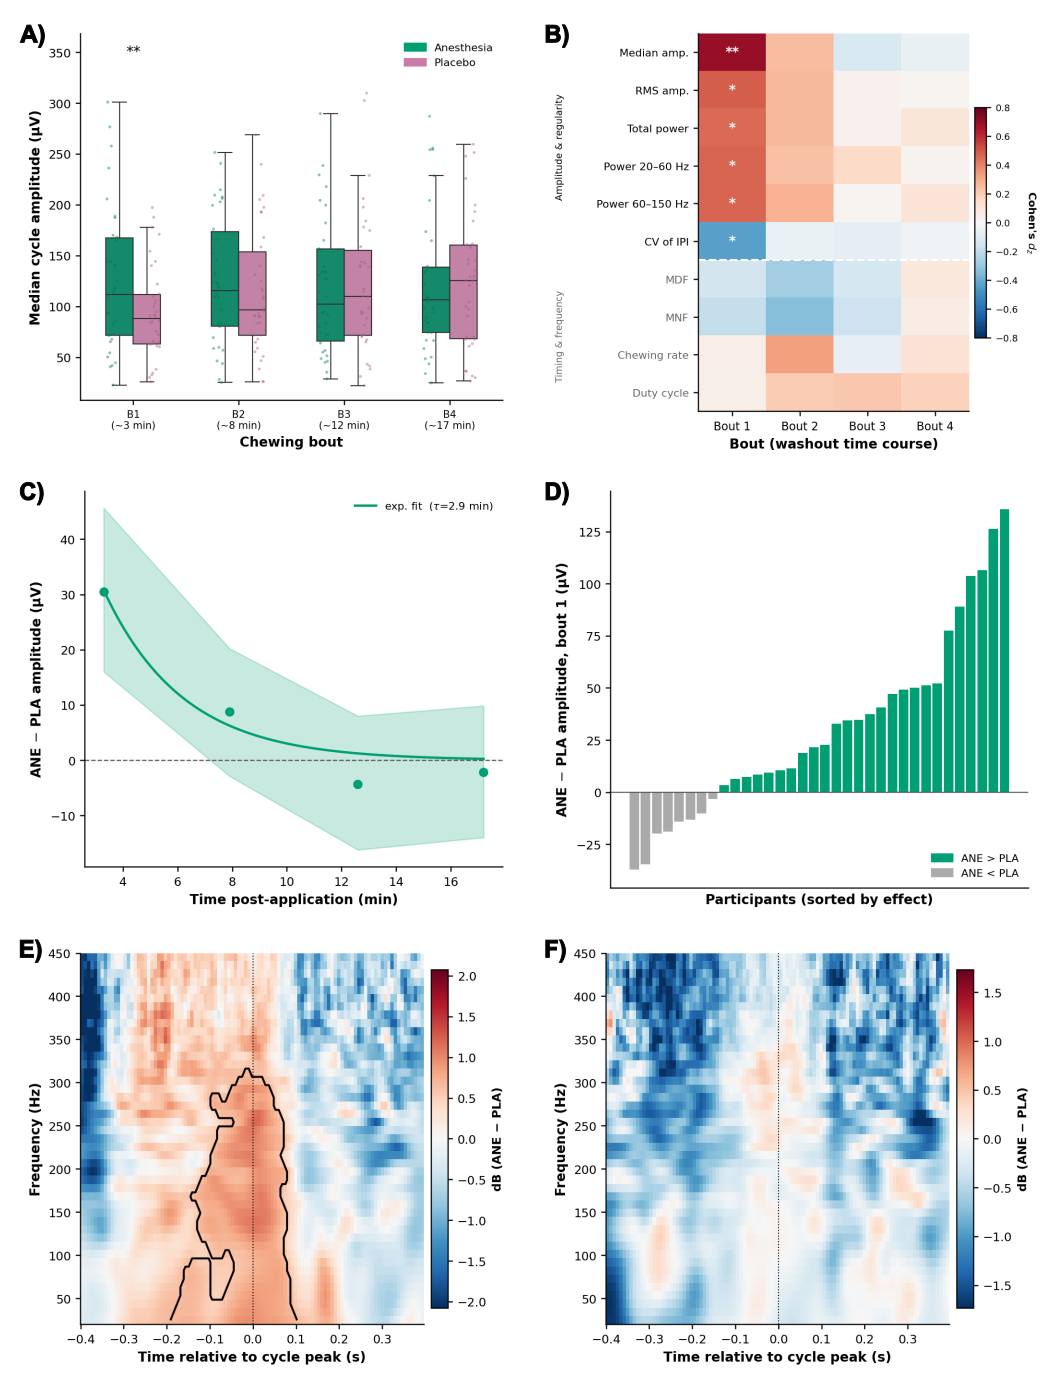
\includegraphics[width=\linewidth]{figures/fig1.png}
\caption{\textbf{Transient sensorimotor gain compensation under masticatory
anesthesia ($N$\,=\,34).}
\textbf{(A)} Median cycle amplitude (\textmu{}V) and \textbf{(B)} coefficient
of variation of the inter-peak interval (CV\textsubscript{IPI}) for
anesthesia (green) and placebo (lilac) across chewing bouts~1--4.
Boxes show median and interquartile range; individual participants overlaid as
jittered points.
Effect size ($d_z$) and FDR-corrected significance are labelled above bout~1
(**: $p_{\text{FDR}}$\,<\,0.01; *: $p_{\text{FDR}}$\,<\,0.05;
Benjamini--Hochberg~\cite{Benjamini1995} across 11~metrics).
\textbf{(C)} Effect-size heatmap ($d_z$, ANE\,$-$\,PLA) for all EMG metrics
(rows) and bouts~1--4 (columns).
White asterisks mark cells surviving FDR correction at bout~1
($p_{\text{FDR}}$\,<\,0.05).
Amplitude and regularity metrics (upper block, black labels) show a transient
gain at bout~1 that converges to zero by bouts~3--4; timing and frequency
metrics (lower block, grey labels) show no effect at any bout.
\textbf{(D)} ANE\,$-$\,PLA difference in median cycle amplitude across bouts
($\approx$\,3, 7.5, 12, and 17~min post-application; error bars: 95\%
bootstrap CI).
Solid curve: exponential decay fit ($\tau$\,$\approx$\,2.9~min), consistent
with topical lidocaine pharmacokinetics~\cite{vonGunten2019}.
\textbf{(E)} Amplitude difference at bout~1 per participant, sorted by
magnitude; green bars: ANE\,$>$\,PLA; grey bars: ANE\,$<$\,PLA.
76\% of participants (26/34) showed greater amplitude under anesthesia
(Wilcoxon $p$\,=\,0.0003).
\textbf{(F)} Grand-average anesthesia-minus-placebo Morlet scalograms
(20--450~Hz; $x$-axis: time relative to cycle peak) at bout~1 (top) and
bout~4 (bottom).
Black contour: significant cluster at bout~1 (cluster-based permutation
test~\cite{Maris2007}; $p$\,=\,0.036; $\approx$\,30--300~Hz,
$-$0.15 to $+$0.1~s relative to cycle peak).
No significant cluster at bout~4 ($p_{\min}$\,=\,0.59).}
\label{fig:main}
\end{figure}

\section*{Methods}

% ─────────────────────────────────────────────────────────────────────────────
\subsection*{Participants and ethics}
% ─────────────────────────────────────────────────────────────────────────────

Data were collected as part of a previously published study~\cite{espinoza2025}.
Thirty-six healthy adults (18--35~years; natural dentition; no dental pain,
temporomandibular disorder diagnosis, or medications affecting neuromuscular
function) participated.
All procedures were approved by the Ethics Committee of the School of Dentistry,
Universidad de Valpara\'{i}so (registration code POSTG-06-22) and conducted in
accordance with the Declaration of Helsinki.
Written informed consent was obtained from all participants before inclusion;
the present secondary analysis falls within the scope of that approval.

% ─────────────────────────────────────────────────────────────────────────────
\subsection*{Study design and anesthesia protocol}
% ─────────────────────────────────────────────────────────────────────────────

The parent study used a 2\,$\times$\,2 within-subject crossover design crossing
chewing (chewing vs.\ no-chewing) with anesthesia condition (anesthesia vs.\
placebo), counterbalanced in two blocks (R1: anesthesia block first; R2: placebo
block first).
The present analysis focuses exclusively on the chewing blocks.
At the start of each chewing block, the experimenter applied one dose of either
topical lidocaine (10\% pump spray) or a matched placebo spray (identical
excipients and taste, no active agent) to the mucosa and periodontal tissues
ipsilateral to the non-chewing side.
No reapplication occurred during the block.
Participants then completed four 60-second chewing bouts with a standardised
food item, separated by approximately 4.5-minute rest intervals, yielding bout
onset times of approximately 3, 7.5, 12, and 17~minutes post-application
per condition.

% ─────────────────────────────────────────────────────────────────────────────
\subsection*{EMG recording}
% ─────────────────────────────────────────────────────────────────────────────

Electrophysiological data were recorded continuously with a BioSemi ActiveTwo
system (BioSemi, Amsterdam, Netherlands) at 1024~Hz from 64 scalp electrodes
and 8 external electrodes (ExG1--8).
Masseter EMG was captured from ExG5--8 using Ag/AgCl electrodes positioned over
the masseter belly in a bipolar configuration following established surface EMG
methodology~\cite{deLuca1997}:
left bipolar pair (ExG5\,$-$\,ExG6) and right bipolar pair (ExG7\,$-$\,ExG8).

% ─────────────────────────────────────────────────────────────────────────────
\subsection*{Signal processing}
% ─────────────────────────────────────────────────────────────────────────────

EMG processing was implemented in Python~3.10 using NumPy, SciPy~\cite{SciPy2020},
and custom modules (analysis code will be deposited at a public repository
upon acceptance; available from the corresponding author on request).
Raw BDF files were processed at the original 1024~Hz sampling rate without
resampling; resampling was avoided to preserve spectral content up to 450~Hz and
prevent aliasing artefacts in the median frequency estimate.
The bipolar derivations were computed as described above.
Signals were band-pass filtered between 20 and 450~Hz using a zero-phase
4th-order Butterworth filter.
Line-frequency noise and harmonics (50, 100, 150, and 200~Hz) were removed with
the Zapline-plus algorithm~\cite{Pyzaplineplus}, which attenuates narrowband
interference without distorting the spectrum at adjacent frequencies, unlike
conventional notch filters.
For each participant, the recording side (left or right) with EMG exhibiting
physiological median frequency (55--170~Hz) and chewing rate (0.6--2.6~Hz)
in both conditions, and with the higher signal-to-noise ratio, was selected for
analysis.
Two participants (M3, M7) were excluded for confirmed dead electrode
artefact in one condition.

% ─────────────────────────────────────────────────────────────────────────────
\subsection*{Cycle detection and feature extraction}
% ─────────────────────────────────────────────────────────────────────────────

Chewing bouts (60~s duration; onset at event code~1) were segmented from the
continuous recording.
Individual masticatory cycles were detected by computing a 100-ms RMS envelope
of the full-wave-rectified bipolar signal, normalising it to a rest-period
$z$-score ($z = (\text{env} - \mu_{\text{rest}}) / \sigma_{\text{rest}}$), and
identifying peaks in the $z$-score trace above the within-bout 50th percentile
with a minimum inter-peak distance of 0.4~s (SciPy~\cite{SciPy2020}).
Using a rest-normalised relative threshold rather than a fixed amplitude cutoff
ensures equivalent detection sensitivity across conditions regardless of signal
magnitude.
To verify that cycle detection was not differentially biased by the amplitude
difference between conditions, we confirmed that the mean number of cycles
detected per bout was equivalent between anesthesia and placebo at every bout
(bout~1: $\bar{n}$\,=\,87.8 vs.\ 87.1 cycles; bouts~2--4: differences
$\leq$\,3 cycles; no paired test approached significance).

Per-bout, per-participant features were extracted: median cycle amplitude
(\textit{med\_amp}), defined as the within-bout median of the instantaneous
amplitude of the full-wave-rectified signal at each detected cycle peak time;
RMS amplitude, total signal power, power in 20--60~Hz and
60--150~Hz bands (Welch method), median frequency (MDF) and mean frequency (MNF)
from the full power spectral density, chewing rate (cycles per second),
coefficient of variation of the inter-peak interval (CV\textsubscript{IPI}), and
duty cycle.
Cycle-locked time-frequency maps were computed by epoching the bipolar signal at
$[-0.4, +0.4]$~s around each detected peak and applying Morlet wavelet
convolution at 30 logarithmically spaced frequencies from 20 to 450~Hz
(wavelet cycles\,=\,7).

% ─────────────────────────────────────────────────────────────────────────────
\subsection*{Statistical analysis}
% ─────────────────────────────────────────────────────────────────────────────

All inferential tests used $N$\,=\,34 participants.
Within each chewing bout, the anesthesia-placebo difference for each metric was
tested with a two-sided paired Wilcoxon signed-rank test~\cite{Pingouin}.
Multiple comparisons across 11 metrics within each bout were controlled by the
Benjamini--Hochberg false-discovery rate (FDR) procedure~\cite{Benjamini1995}.
FDR correction was applied within each bout separately, consistent with the
a~priori hypothesis that bout~1 would carry the primary pharmacological effect;
the four bout comparisons were treated as planned time-points (not as a joint
family requiring cross-bout correction).
Effect sizes are reported as paired Cohen's $d_z$~\cite{Cohen1988}.
A post-hoc sensitivity analysis (paired $t$ equivalent, $\alpha$\,=\,0.05
two-tailed, $1-\beta$\,=\,0.80, $N$\,=\,34) indicated that the study was
powered to detect effects of $d_z$\,$\geq$\,0.49; the primary bout~1 effect
($d_z$\,=\,0.695) substantially exceeds this threshold, while the null effects
at bouts~3--4 ($d_z$\,$\leq$\,0.10) are well below it, consistent with the
TOST-confirmed equivalence at those bouts.
Session-averaged equivalence of timing metrics was assessed with two one-sided
tests (TOST) at an equivalence bound of $|d|$\,=\,0.5~\cite{Lakens2017};
this bound corresponds to a medium effect size and represents a conventional
threshold for practical equivalence that is accepted as meaningful in the
sensorimotor literature~\cite{Lakens2017}.
The condition\,$\times$\,bout interaction was tested with a repeated-measures
ANOVA using Pingouin~\cite{Pingouin} with Greenhouse--Geisser sphericity
correction.
Cycle-locked TF maps were compared between conditions by a one-sample
cluster-based permutation test on the paired ANE\,$-$\,PLA difference map
(5\,000 permutations; cluster-forming threshold $t$ at $p$\,=\,0.05)~\cite{Maris2007}.
Crossover confound analyses used a mixed ANOVA (condition\,$\times$\,counterbalancing
arm) at bout~1 and an unpaired Mann--Whitney test for residual carryover.
As an exploratory analysis, bilateral masseter synchrony was quantified for
participants with physiologically valid signals on both left and right sides
($N$\,=\,31; median frequency 45--200~Hz and chewing rate 0.4--2.8~Hz in
both conditions).
Within each bout, the Pearson correlation between left and right masseter
RMS envelopes (50-ms window) was computed as a measure of bilateral temporal
coupling, and the amplitude asymmetry index (L\,$-$\,R)/(L\,$+$\,R) was
derived from the mean envelope amplitudes.
Bilateral metrics were compared between conditions using paired Wilcoxon tests
(FDR-corrected) and a 2\,$\times$\,4 repeated-measures ANOVA
(condition\,$\times$\,bout).


% ─────────────────────────────────────────────────────────────────────────────
% DATA AVAILABILITY
% ─────────────────────────────────────────────────────────────────────────────
\section*{Data availability}
The dataset analysed here is the same as that of the parent
study~\cite{espinoza2025}.
The original recordings and derived EMG measures produced for the present
analysis will be deposited at [REPOSITORY/DOI -- to be assigned upon acceptance].
Analysis code (Python~3.10) is archived at
[CODE REPOSITORY -- to be assigned upon acceptance].

% ─────────────────────────────────────────────────────────────────────────────
% SECONDARY DATA STATEMENT
% ─────────────────────────────────────────────────────────────────────────────
\section*{Secondary data statement}
The data analysed here were acquired as part of a previously published
study~\cite{espinoza2025} and are re-analysed here for a distinct purpose.
That study used a 2\,$\times$\,2 within-subject design crossing chewing with
dental anesthesia and reported behavioral and EEG outcomes; the present work
constitutes a secondary analysis focused on the surface masseter electromyogram,
which was not analysed as a primary outcome in the parent study.
No new data were collected.
Behavioral data from the parent study are referenced here only as contextual
information and are not re-reported as original findings.

% ─────────────────────────────────────────────────────────────────────────────
% ETHICS
% ─────────────────────────────────────────────────────────────────────────────
\section*{Ethics declarations}
All procedures were approved by the Ethics Committee of the School of Dentistry,
Universidad de Valpara\'{i}so (registration code POSTG-06-22) and conducted in
accordance with the Declaration of Helsinki.
Written informed consent was obtained from all participants; the present
secondary analysis falls within the scope of that approval and consent.

% ─────────────────────────────────────────────────────────────────────────────
% COMPETING INTERESTS
% ─────────────────────────────────────────────────────────────────────────────
\section*{Competing interests}
The authors declare no competing interests.

% ─────────────────────────────────────────────────────────────────────────────
% AUTHOR CONTRIBUTIONS (CRediT)
% ─────────────────────────────────────────────────────────────────────────────
\section*{Author contributions}
S.E.: Conceptualisation, Data curation, Formal analysis, Investigation,
Methodology, Software, Visualisation, Writing -- original draft,
Writing -- review \& editing.
D.M.-E.: Formal analysis (pharmacological), Investigation, Writing -- review
\& editing.
L.M.-O.: Investigation, Resources, Writing -- review \& editing.
W.E.-D.: Conceptualisation, Funding acquisition, Methodology, Supervision,
Writing -- review \& editing.
All authors read and approved the final manuscript.

% ─────────────────────────────────────────────────────────────────────────────
% ACKNOWLEDGMENTS
% ─────────────────────────────────────────────────────────────────────────────
\section*{Acknowledgments}
[To be completed: funding sources, institutional support, participant
acknowledgments.]

% ─────────────────────────────────────────────────────────────────────────────
% AI USAGE STATEMENT
% ─────────────────────────────────────────────────────────────────────────────
\section*{AI usage statement}
Manuscript drafting was assisted using Claude (Anthropic) via the Claude Code
interface.
All statistical analyses, data interpretations, and scientific conclusions were
verified by the authors.
Final responsibility for the accuracy and integrity of this work rests with
the authors.


\newpage
\bibliography{biblio}
\newpage
{\LARGE\textbf{Supplementary Material}}
% ─────────────────────────────────────────────────────────────────────────────
% SUPPLEMENTARY MATERIAL
% 3 figures (sup1–sup3) + 3 tables
% Counter \suppfigure increments for both figures and tables (S1–S6).
% ─────────────────────────────────────────────────────────────────────────────

% ─── S1: Experimental paradigm ───────────────────────────────────────────────
\begin{figure}[!h]
\centering
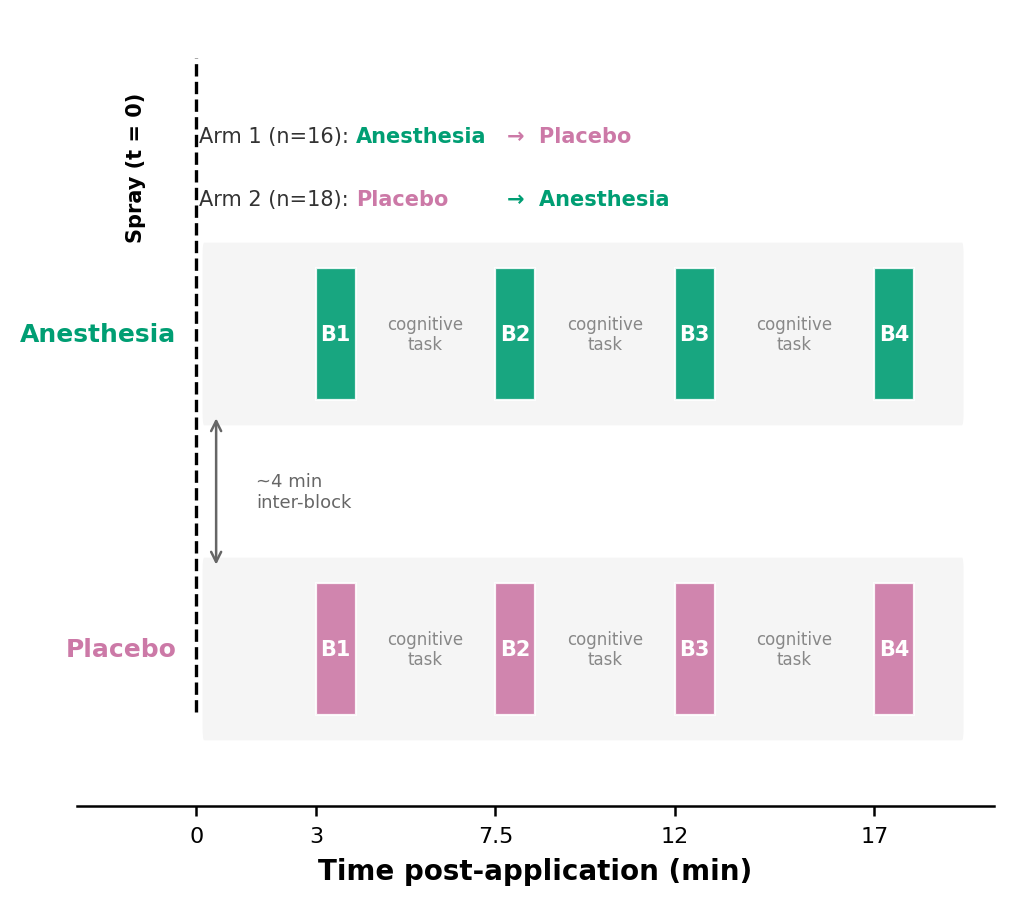
\includegraphics[width=\linewidth]{figures/sup1.png}
\refstepcounter{suppfigure}\label{fig:supp_paradigm}
\caption{\textbf{Supplementary Fig.~\thesuppfigure~$|$~Within-session
crossover design.}
Each experimental session comprised two chewing blocks separated by
$\approx$\,4~min.
Arm~1 ($n$\,=\,16): anesthesia block first, then placebo;
Arm~2 ($n$\,=\,18): placebo first, then anesthesia.
Each block began with a single spray application of topical lidocaine~10\%
or matched placebo (saline) at $t$\,=\,0; four 60-second chewing bouts
(B1--B4) commenced at approximately 3, 7.5, 12, and 17~min post-application.
Cognitive tasks (auditory oddball and 2-back) were performed between
consecutive bouts; these are indicated by the grey labels between blocks.
The short intra-session inter-block interval ($\approx$\,4~min) is sufficient
for pharmacological reversal: the placebo bout-1 is statistically equivalent
between arms (Supplementary Table~S3; carryover $p$\,=\,0.379; no period
effect $p$\,=\,0.134).
Green blocks: anesthesia condition; lilac blocks: placebo condition.}
\end{figure}

% ─── S2: Signal quality and participant inclusion ─────────────────────────────
\begin{figure}[!h]
\centering
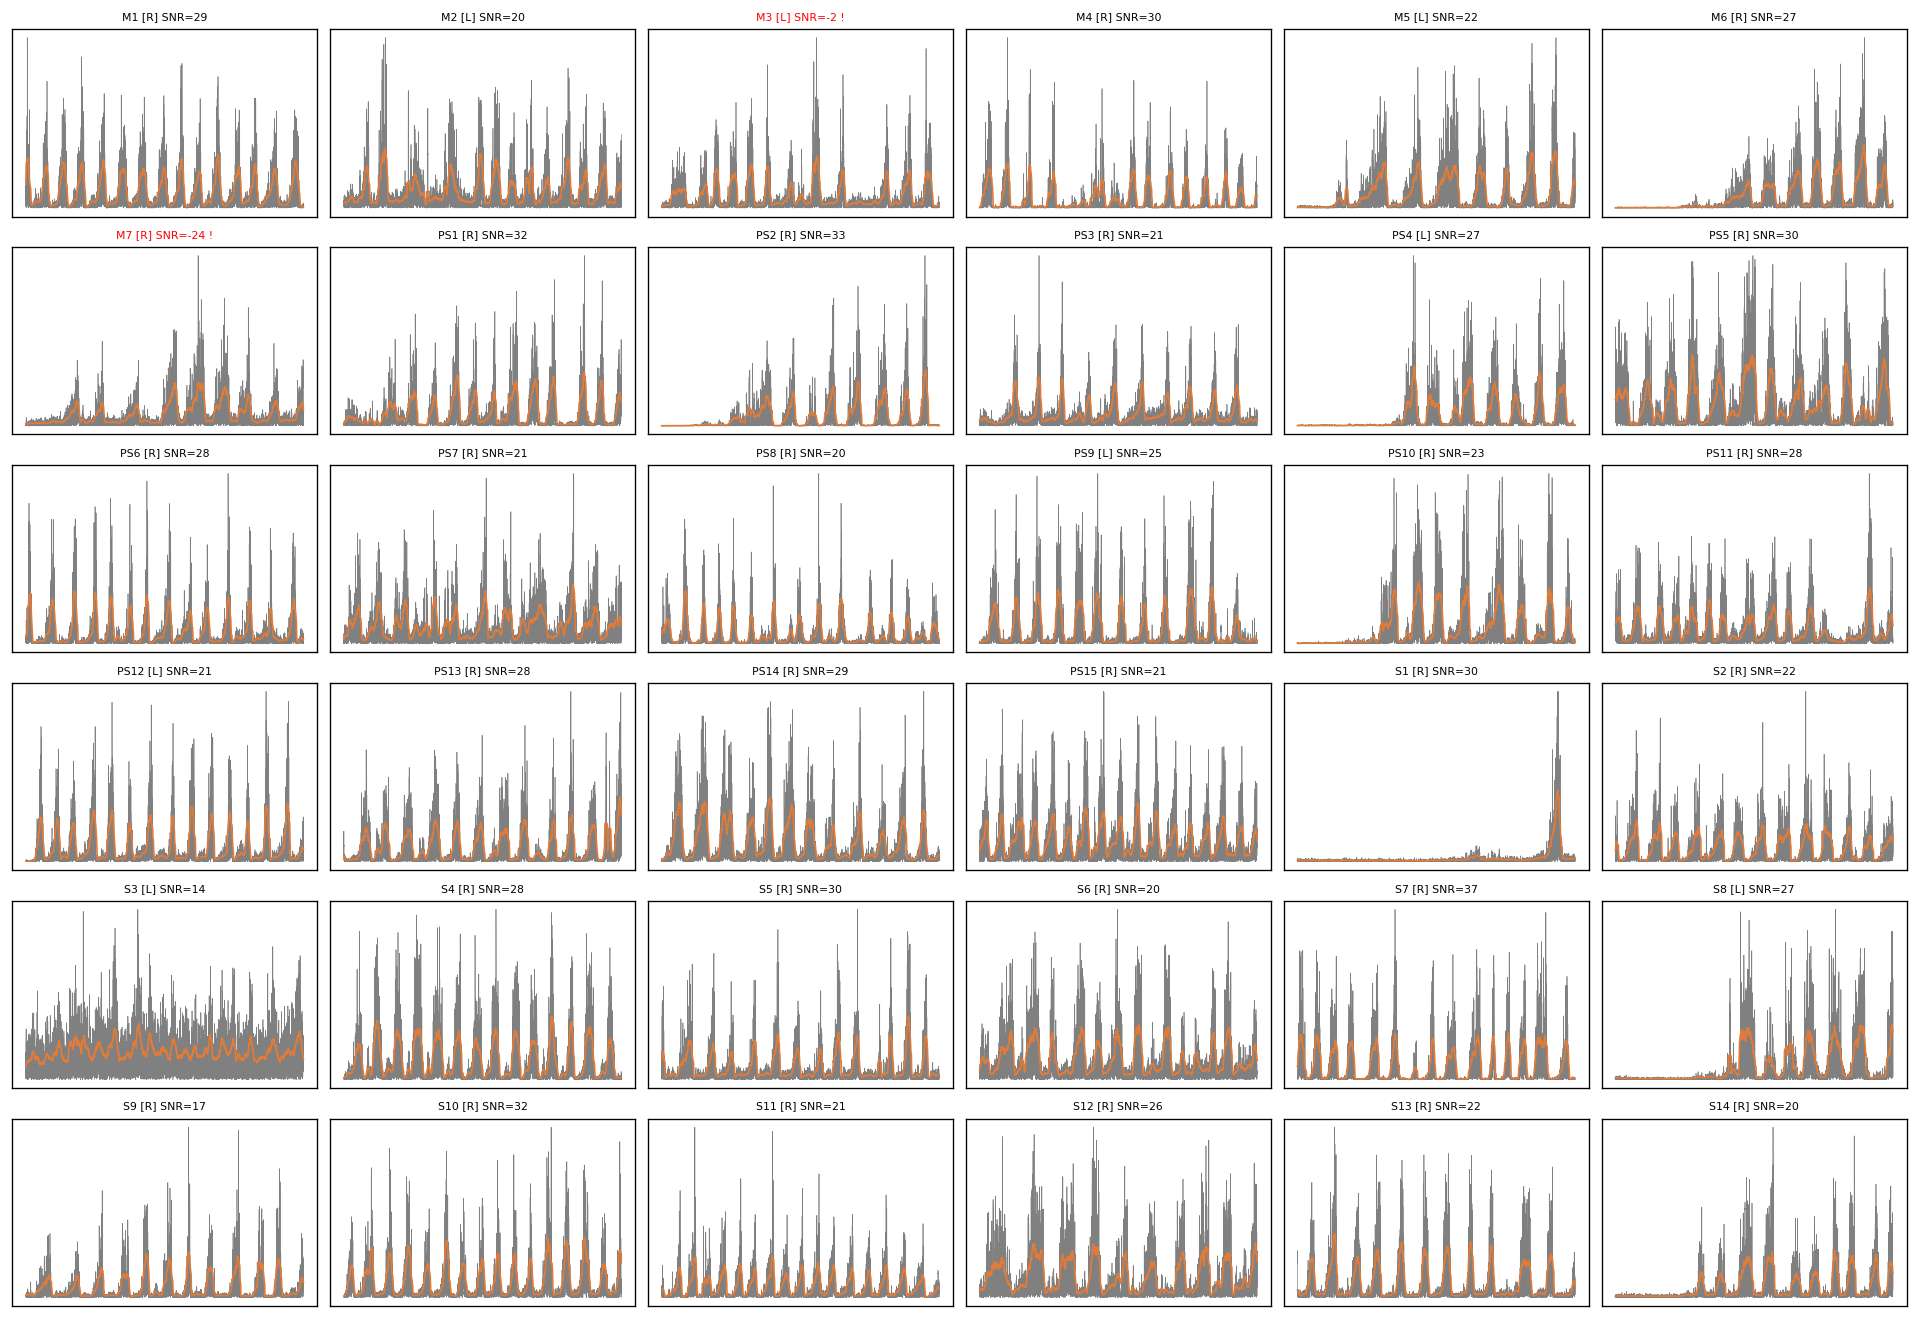
\includegraphics[width=\linewidth]{figures/sup2.png}
\refstepcounter{suppfigure}\label{fig:supp_qc}
\caption{\textbf{Supplementary Fig.~\thesuppfigure~$|$~Signal quality and
participant inclusion.}
Bipolar masseter EMG quality-control (QC) grid for all 36 recorded
participants.
Each panel shows the rectified bipolar waveform during the first 8~s of
chewing bout~1 (anesthesia and placebo overlaid) with detected cycle peaks
marked.
Two participants (M3, M7) are excluded from all analyses due to a dead
electrode in one condition, confirmed by near-zero amplitude and flat power
spectrum in the affected condition (SNR\,$<$\,3~dB).
Included: $N$\,=\,34; excluded: $N$\,=\,2.
Side selection (left or right masseter) was based on signal quality and
confirmed by automated SNR criterion.}
\end{figure}

% ─── S3: Effect-size overview and magnitude of change ────────────────────────
\begin{figure}[!h]
\centering
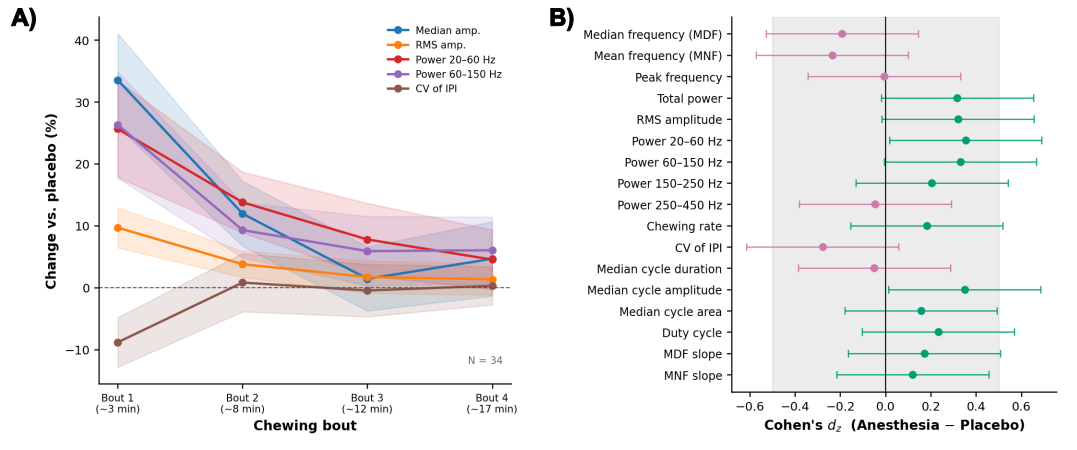
\includegraphics[width=\linewidth]{figures/sup3.png}
\refstepcounter{suppfigure}\label{fig:supp_effectsize}
\caption{\textbf{Supplementary Fig.~\thesuppfigure~$|$~Effect-size overview
and normalised magnitude of anesthesia-induced changes.}
\textbf{(A)} Percentage change relative to placebo
[(ANE\,$-$\,PLA)\,/\,$|$PLA$|$\,$\times$\,100] across chewing bouts~1--4 for
the five metrics with FDR-corrected significance at bout~1 (median amplitude,
RMS amplitude, power 20--60~Hz, power 60--150~Hz, CV\textsubscript{IPI}).
All metrics show a transient effect peaking at bout~1 ($\approx$\,3~min
post-application) that converges toward zero by bouts~3--4, consistent with
lidocaine pharmacokinetic washout.
Error bands: $\pm$\,SEM.
\textbf{(B)} Forest plot of Cohen's $d_z$ (ANE\,$-$\,PLA) for all 11 EMG
metrics, session-averaged across bouts~1--4.
Dots: point estimate; horizontal bars: 95\% CI ($\pm$\,1.96\,/\,$\sqrt{N}$).
The grey band marks the equivalence zone ($|d_z|$\,<\,0.5).
Session-averaged amplitude metrics are non-significant after FDR correction
(bout-1 effect diluted by within-session washout); timing and frequency
metrics lie within the equivalence band at all bouts, confirming the
gain--timing dissociation described in the main text.
$N$\,=\,34.}
\end{figure}

% ─────────────────────────────────────────────────────────────────────────────
% SUPPLEMENTARY TABLES
% ─────────────────────────────────────────────────────────────────────────────

% ─── S4: Session-averaged equivalence (TOST) ─────────────────────────────────
\refstepcounter{suppfigure}\label{fig:supp_tost}
\begin{table}[!h]
\centering
\caption{\textbf{Supplementary Table~\thesuppfigure~$|$~Session-averaged
anesthesia vs.\ placebo comparison (all four bouts pooled, $N$\,=\,34).}
Paired Cohen's $d_z$, Wilcoxon $p$, FDR-corrected $p$~\cite{Benjamini1995},
and two one-sided test (TOST) result at equivalence bound $|d|\,=\,0.5$~\cite{Lakens2017}.
TOST\,=\,Equiv.: both one-sided tests $p$\,<\,0.05.
Timing metrics satisfy or approach equivalence; amplitude metrics are
non-significant after FDR correction but do not satisfy equivalence,
consistent with the diluted transient effect described in the main text.}
\label{tab:tost_full}
\begin{tabular}{llrrrr}
\toprule
Category & Metric & $d_z$ & Wilcoxon $p$ & FDR $p$ & TOST ($|d|\leq0.5$) \\
\midrule
\multirow{5}{*}{Timing / frequency}
 & Median frequency (MDF)     & $-$0.191 & 0.186 & 0.376 & Equiv. \\
 & Mean frequency (MNF)       & $-$0.235 & 0.138 & 0.336 & Marginal ($p$\,=\,0.066) \\
 & Chewing rate (Hz)          & $+$0.182 & 0.278 & 0.415 & Equiv. \\
 & Cycle duration (s)         & $-$0.049 & 0.758 & 0.806 & Equiv. \\
 & Duty cycle                 & $+$0.233 & 0.221 & 0.376 & Marginal ($p$\,=\,0.065) \\
\midrule
\multirow{6}{*}{Amplitude / power}
 & Median cycle amplitude     & $+$0.349 & 0.011 & 0.181 & Not equiv. \\
 & RMS amplitude              & $+$0.320 & 0.109 & 0.336 & Not equiv. \\
 & Total power                & $+$0.317 & 0.109 & 0.336 & Not equiv. \\
 & Power 20--60~Hz            & $+$0.354 & 0.121 & 0.336 & Not equiv. \\
 & Power 60--150~Hz           & $+$0.331 & 0.109 & 0.336 & Not equiv. \\
 & CV inter-peak interval     & $-$0.278 & 0.046 & 0.336 & Not equiv. \\
\bottomrule
\end{tabular}
\end{table}

% ─── S5: Bout-resolved statistics ────────────────────────────────────────────
\refstepcounter{suppfigure}\label{fig:supp_boutstats}
\begin{table}[!h]
\centering
\caption{\textbf{Supplementary Table~\thesuppfigure~$|$~Bout-resolved
anesthesia vs.\ placebo effect sizes ($d_z$, paired Cohen's~$d$~\cite{Cohen1988})
for key metrics, $N$\,=\,34.}
FDR $p$ shown only for bout~1 (Benjamini--Hochberg~\cite{Benjamini1995} across
11 metrics); asterisks denote FDR-corrected significance (**\,$p$\,<\,0.01;
*\,$p$\,<\,0.05).
Interaction $p$: Greenhouse--Geisser-corrected condition\,$\times$\,bout
repeated-measures ANOVA~\cite{Pingouin}.
Positive $d_z$ = ANE\,$>$\,PLA; negative $d_z$ for CV\textsubscript{IPI}
indicates greater regularity under anesthesia.}
\label{tab:bout_stats}
\begin{tabular}{lrrrrrr}
\toprule
Metric & \multicolumn{4}{c}{$d_z$ by bout} & FDR $p$ (b1) & Inter. $p$ \\
\cmidrule(lr){2-5}
       & Bout 1 & Bout 2 & Bout 3 & Bout 4 & & \\
\midrule
\textit{Amplitude}\\
\quad Median cycle amplitude & $+$0.695** & $+$0.248 & $-$0.120 & $-$0.058 & 0.0035 & 0.0010 \\
\quad RMS amplitude          & $+$0.487*  & $+$0.257 & $+$0.034 & $+$0.024 & 0.0132 & 0.130  \\
\quad Total power            & $+$0.456*  & $+$0.261 & $+$0.032 & $+$0.095 & 0.0132 & 0.260  \\
\quad Power 60--150~Hz       & $+$0.463*  & $+$0.281 & $+$0.025 & $+$0.100 & 0.0189 & 0.238  \\
\quad Power 20--60~Hz        & $+$0.467*  & $+$0.231 & $+$0.151 & $+$0.027 & 0.0274 & 0.445  \\
\midrule
\textit{Regularity}\\
\quad CV\textsubscript{IPI}  & $-$0.434*  & $-$0.051 & $-$0.070 & $-$0.026 & 0.0415 & 0.057  \\
\midrule
\textit{Timing (all non-significant; TOST-equivalent at all bouts)}\\
\quad Median frequency (MDF) & $-$0.147 & $-$0.275 & $-$0.139 & $+$0.085 & 0.621 & 0.485 \\
\quad Chewing rate           & $+$0.054 & $+$0.331 & $-$0.069 & $+$0.113 & 0.919 & 0.230 \\
\quad Duty cycle             & $+$0.045 & $+$0.203 & $+$0.213 & $+$0.185 & 0.909 & 0.848 \\
\bottomrule
\end{tabular}
\end{table}

% ─── S6: Robustness ──────────────────────────────────────────────────────────
\refstepcounter{suppfigure}\label{fig:supp_robust}
\begin{table}[!h]
\centering
\caption{\textbf{Supplementary Table~\thesuppfigure~$|$~Robustness of the
bout-1 anesthesia effect across inclusion cohorts.}
Bout-1 paired Cohen's $d_z$, Wilcoxon $p$, percentage of participants with
ANE\,$>$\,PLA, and condition\,$\times$\,bout RM-ANOVA interaction $p$
(Greenhouse--Geisser corrected) for median cycle amplitude under four
alternative inclusion thresholds.
The attenuation at $N$\,=\,36 is attributable to M3 and M7 (dead electrode in
one condition), whose inclusion approximately halves the effect size while the
paired test remains significant ($p$\,=\,0.002), confirming the
quality-based exclusion criterion.}
\label{tab:robustness}
\begin{tabular}{lrrrrr}
\toprule
Cohort & $N$ & $d_z$ & Wilcoxon $p$ & \%~ANE$>$PLA & cond$\times$bout $p$ \\
\midrule
QC automatic                     & 34 & 0.69 & 0.0003 & 76\% & 0.0004 \\
Lista~30                         & 30 & 0.68 & 0.001  & 77\% & 0.001  \\
Lista~32                         & 32 & 0.65 & 0.001  & 75\% & 0.001  \\
All (incl.\ M3/M7, $N$\,=\,36)  & 36 & 0.26 & 0.002  & 72\% & 0.061  \\
\bottomrule
\end{tabular}
\end{table}

\FloatBarrier
\end{document}
